\section{Future Work}
\frame{Future Work}

\begin{frame}{NBL control design through contacts}
    \small
    \begin{columns}
    \begin{column}{0.5\linewidth}
        \begin{itemize}
            \item The NBL technique can be extended to more complicated systems
            such as contact-rich systems
            \item The objective is to design robust data-driven controllers that
            exhibit desired properties and account for uncertainties in the hybrid
            dynamical model
        \end{itemize}
        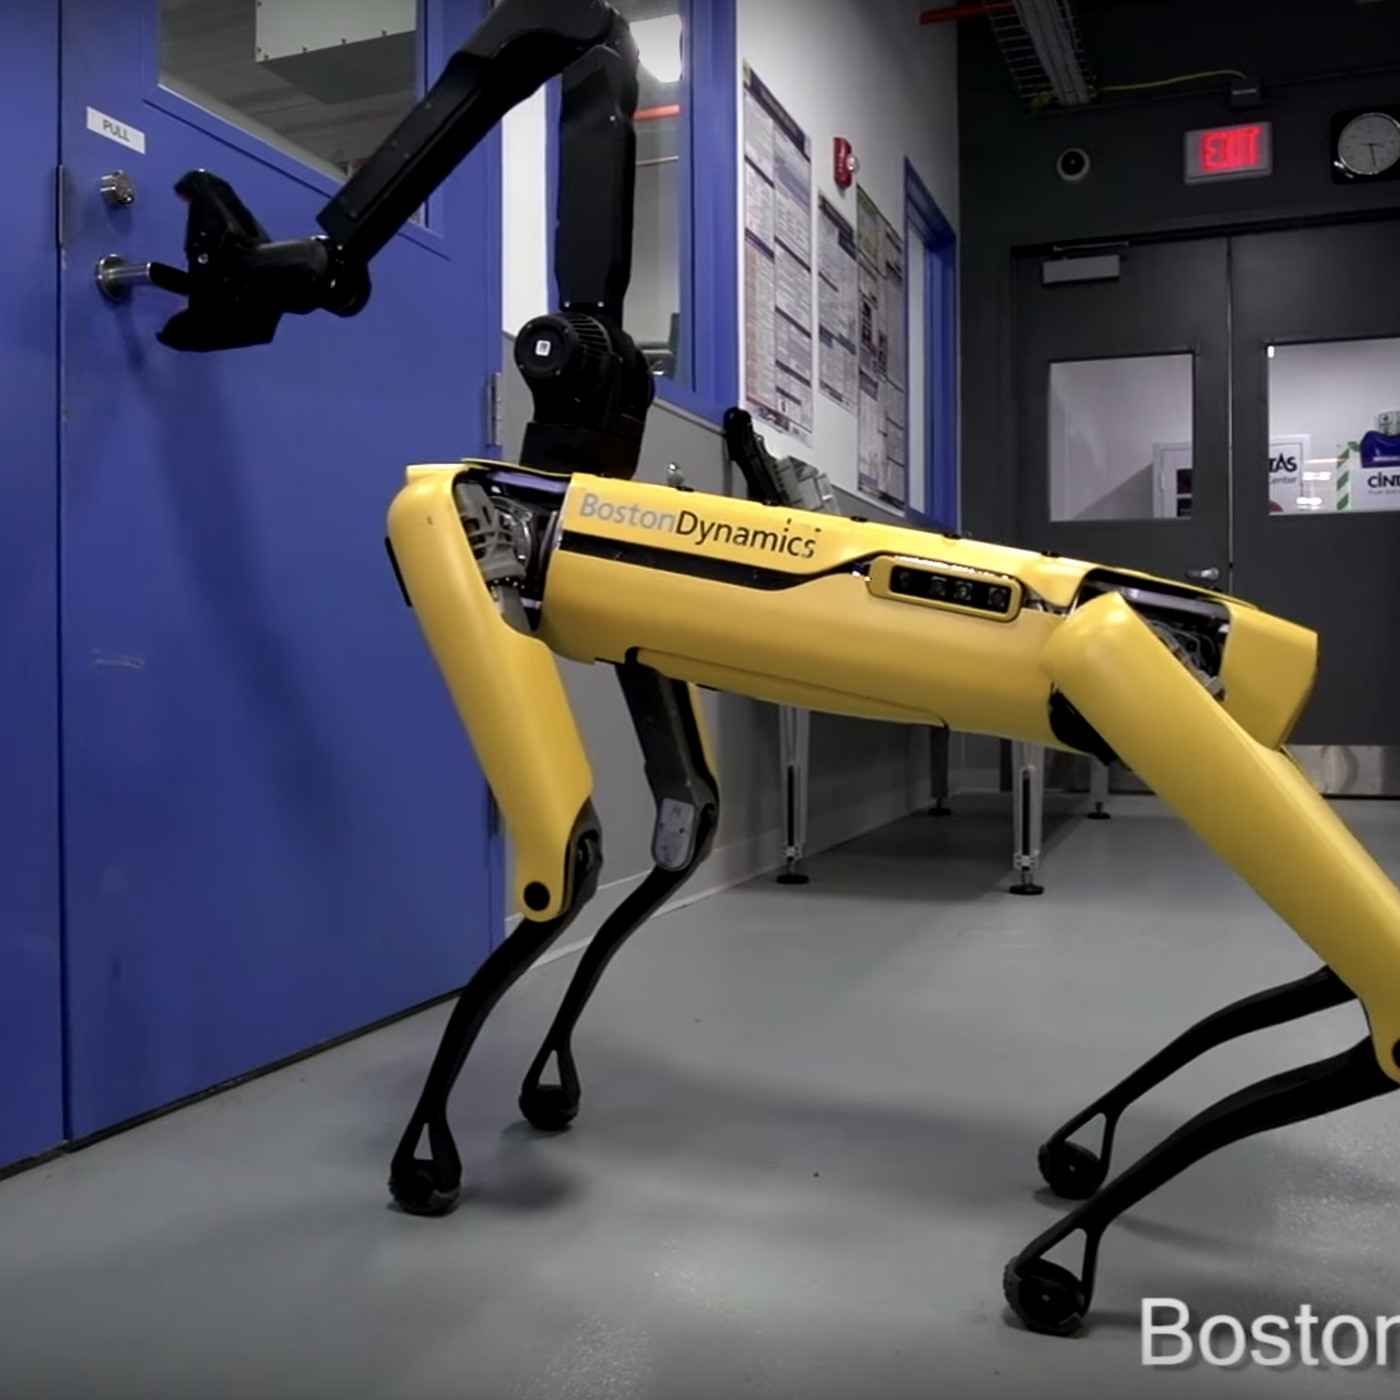
\includegraphics[width=0.4\linewidth, center]{hound.jpeg}
    \end{column}
    \begin{column}[t]{0.5\linewidth}
        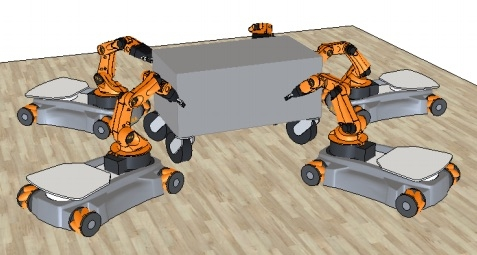
\includegraphics[width=0.85\linewidth,]{cm1.jpg}
        % \vspace{-1.24cm}
        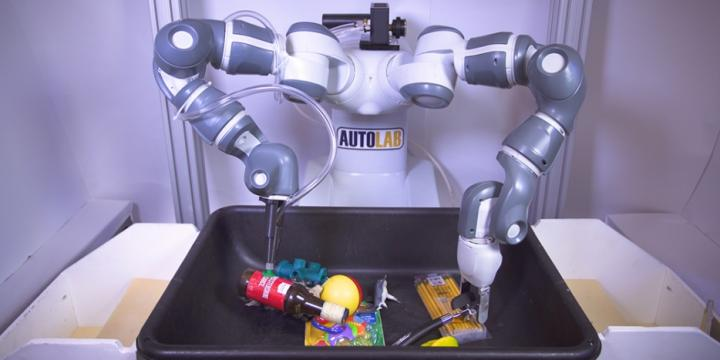
\includegraphics[width=0.85\linewidth]{gripper.jpg}
    \end{column}
    \end{columns}
    \footnotetext[1]{Antonio Petitti, Antonio Franchi, Donato Di Paola, Alessandro Rizzo. Decentralized Motion Control
    for Cooperative Manipulation with a Team of Networked Mobile Manipulators. 2016 IEEE Interna-
    tional Conference on Robotics \& Automation (ICRA), May 2016, Stockholm, Sweden. pp. 441-446.}
\end{frame}

\begin{frame}{Linear Complementarity Problem (LCP)}
    \begin{itemize}
        \item Contacts, impacts and Coulomb friction are modelled through linear complementarity problems (LCP) given by the following convex optimization problem
    \end{itemize}
    \begin{columns}
        \begin{column}{0.4\linewidth}
            \begin{exampleblock}{Linear Complementarity Problem}
                \small
                \begin{equation*}
                    \begin{aligned}
                        \underset{\xi_n, \xi_t, \Lambda_n, \Lambda_t }{\textrm{minimize}} 
                        &\quad 0 \\
                        \textrm{subject to}
                        &\quad 0 \leq  \begin{pmatrix}
                            \xi_n \\ \xi_t \\ \Lambda_l
                        \end{pmatrix}  \perp  \begin{pmatrix}
                            \Lambda_n \\ \Lambda_r \\ \xi_l
                        \end{pmatrix}  \geq 0,  \\
                        &\quad  \begin{pmatrix}
                            \xi_n \\ \xi_r \\ \Lambda_l
                        \end{pmatrix}  = A  \begin{pmatrix}
                            \Lambda_n \\ \Lambda_r \\ \xi_l
                        \end{pmatrix}  + B 
                    \end{aligned} 
                \end{equation*}
              \end{exampleblock}
        \end{column}
        \begin{column}[]{0.5\linewidth}
            \begin{figure}
                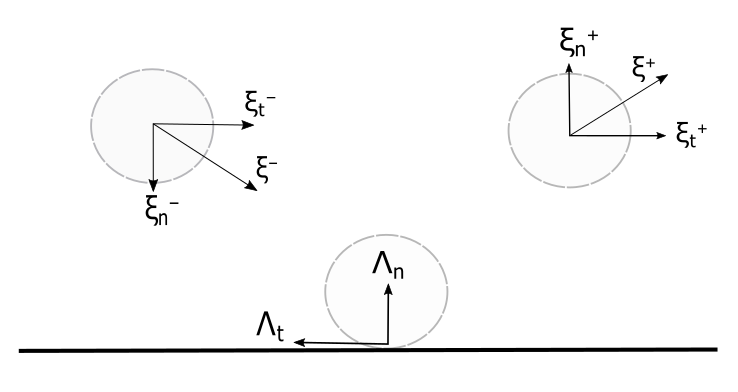
\includegraphics[width=0.9\linewidth]{ball_contact.png}
                    \caption{Bouncing ball contact event}
            \end{figure}
            % \begin{align*}
            %     \Lambda_R &:= µ\Lambda_N + \Lambda_T , \\
            %     \Lambda_L &:= µ\Lambda_N - \Lambda_T , \\
            %     \xi_T &= \xi_R - \xi_L .
            \vspace{-0.2cm}
            \raggedright $\Lambda$ represents contact forces and $\xi$ are the post-contact velocities, in the tangential and normal directions.

        \end{column}
    \end{columns}
\end{frame}

\begin{frame}
    % \begin{itemize}
    %     \item 
    % \end{itemize}
    \begin{exampleblock}{Neural Bayesian Learning with Contacts, Impacts and Coulomb Friction}
        \begin{equation*}
            \begin{aligned}
                \underset{q(\theta) }{\text{min}} 
                &&\quad J(&\phi(t; x_0, u), u) \\
                \text{subject to} 
                &&\quad M(x)\dd x &- h(x, \dot{x}, u) \dd t - \dd \Lambda= 0, \\
                &&\quad u(x; \theta) &= \mathcal{D}\{F(x; \theta)\}, \\
                &&\quad \zeta &\sim \mathcal{N}(\zeta_0, \Sigma_{\zeta}), \\
                &&\quad \theta &\sim q(\theta),
            \end{aligned} 
        \end{equation*}
      \end{exampleblock}
    \raggedright where $M$ is the mass matrix, $h$ holds Coriolis terms and generalized
    forces and $\Lambda$ holds the normal and tangential contact forces on the
    system.
\end{frame}

\begin{frame}{Rimless Wheel}
    \begin{columns}
        \begin{column}{0.4\linewidth}
            \begin{itemize}
               \item The rimless wheel will be used as a test bed for the NBL control design. \\
               \item We will design a robust controller under system parameter uncertainties such as surface friction. 
            \end{itemize}
        \end{column}
        \begin{column}{0.5\linewidth}
            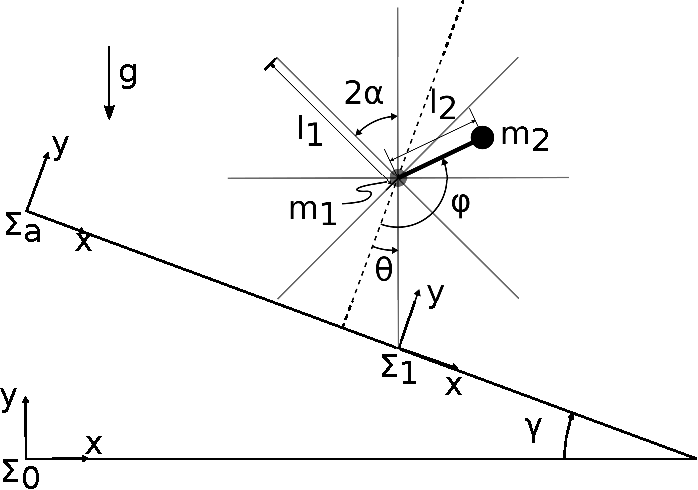
\includegraphics[width=0.9\linewidth]{rimless_wheel.pdf}
        \end{column}
        \end{columns}
    \footnotetext[1]{Sirichotiyakul, Wankun, et al. "Energetically-optimal discrete and continuous stabilization of the rimless wheel with torso." International Design Engineering Technical Conferences and Computers and Information in Engineering Conference. Vol. 59230. American Society of Mechanical Engineers, 2019.}
\end{frame}

\begin{frame}{Schedule}
    \begin{table}[H]
        \centering
        \caption{Schedule}
        % \rowcolors{2}{}{Wheat1}
        \begin{tabular}{|c|c|}
        \toprule
        %   & \multicolumn{2}{c}{Framework} \\
        %   \cmidrule(lr){2-3}
        \textbf{Timeline} & \textbf{Task} \\
        \midrule 
        \midrule
            May - August 2022 & Design and build the rimless wheel \\
            August - September 2022 & Learn deterministic policy of the rimless-wheel \\ 
            October - November 2022 & Learn stochastic policy of the rimless-wheel \\
            November - December 2022 & Submit work to a journal publication \\
            December 2022 - February 2023 & Write dissertation \\
            March - May 2023 & Prepare dissertation presentation and defend \\
        \bottomrule
        \end{tabular}
        \label{tab:training_setup_neuralpbc}
    \end{table}
\end{frame}

\section{Questions?}
\frame{Questions?}